%%
% Please see https://bitbucket.org/rivanvx/beamer/wiki/Home for obtaining beamer.
%%
\documentclass{beamer}

\usetheme{Luebeck}
\usecolortheme{crane}
\setbeamertemplate{section in toc}[ball unnumbered]
\setbeamertemplate{subsection in toc}[ball unnumbered]

\usepackage[T1]{fontenc}
\usepackage{beramono}
\usepackage{graphicx}
\usepackage{hyperref}
\usepackage{pifont}
\usepackage{listings}
\usepackage{xcolor}
\usepackage{multicol}


%\definecolor{darkgreen}{rgb}{0.,0.6,0.}

\newcounter{questionizeIndex}

\newenvironment{questionize}[1][0]{%
    \setbeamercovered{invisible}%
    \setcounter{questionizeIndex}{#1}%
    \begin{itemize}%
}{ %
    \end{itemize}%
}

\newcommand{\question}[2]{%
    % #1: question
    % #2: answer (replaces question)
    \stepcounter{questionizeIndex}%
    \item<\value{questionizeIndex}->%
    \only<\value{questionizeIndex}>{#1}%
    \stepcounter{questionizeIndex}%
    \only<\value{questionizeIndex}->{#2}%
}

\newcommand{\lquestion}[4]{%
    % #1: question label
    % #2: question
    % #3: answer label
    % #4: answer (replaces question)
    \stepcounter{questionizeIndex}%
    \item[\only<\value{questionizeIndex}->{\alt<\value{questionizeIndex}>{#1}{#3}}]<\value{questionizeIndex}->%
    \only<\value{questionizeIndex}>{#2}%
    \stepcounter{questionizeIndex}%
    \only<\value{questionizeIndex}->{#4}%
}

\newcommand{\cquestion}[2]{\question{#2}{\color{#1}{#2}}}

\newcommand{\ctrue}[1]{\cquestion{darkgreen}{#1}}
\newcommand{\cfalse}[1]{\cquestion{red}{#1}}

\newcommand{\ltrue}[1]{\lquestion{\textbf{?}}{#1}{$\checkmark$}{#1}}
\newcommand{\lfalse}[1]{\lquestion{\textbf{?}}{#1}{$\times$}{#1}}

\lstset{
    basicstyle=\footnotesize\ttfamily,
    breaklines=true
}


\hypersetup{%
  colorlinks=true,% hyperlinks will be black
  pdfborderstyle={/S/U/W 1}% border style will be underline of width 1pt
}
\begin{document}

\title{MSiA490 SEC20/28\\ Text Analytics}
\subtitle{Lab 5 - Text Classification}
\author{Timo Wang}
\institute{Northwestern University}
\date{October 15, 2020}

\begin{frame}
    \titlepage
\end{frame}

\begin{frame}{Overview}
    \tableofcontents[hideallsubsections]
\end{frame}

\section{What is classification?}
\begin{frame}
    \frametitle{What is classification?}
    \begin{figure}
        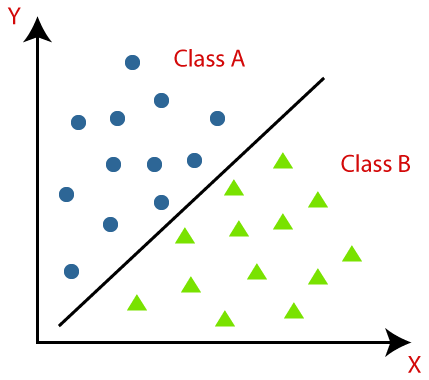
\includegraphics[scale=0.23]{classification}
        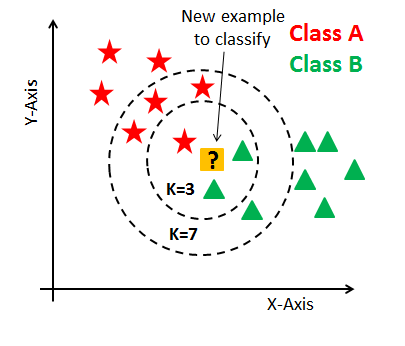
\includegraphics[scale=0.25]{knn_classification}
        \caption{Given a set of feature vectors, e.g. sentence embeddings, word embeddings, bag-of-words, etc., separate them from each other, either linearly (left) or non-linearly (right)}
    \end{figure}
\end{frame}

\section{How do we approach classification?}
\subsection{Simple solution}
\begin{frame}
    \frametitle{How do we approach classification?}
    \framesubtitle{Simple solution}
    Use existing packages/libraries!
    \begin{itemize}
        \item \textbf{scikit-learn} provides both SVM models as well as logistic regression models.
        \item \textbf{FastText} is an alternative tool that also works as command line programs. 
    \end{itemize}
\end{frame}

\subsection{Data preparation}
\begin{frame}
    \frametitle{How do we approach classification?}
    \framesubtitle{Data preparation}
    $\mathbf{X}$: a 2-d array of size $(n, d)$, where $n$ is the number of training examples and $d$ is the size of the feature.\\
    $\mathbf{y}$: a 1-d array of length $n$, where $n$ is the number of training examples.
\end{frame}

\subsection{Model fitting and prediction}
\begin{frame}[containsverbatim]
    \frametitle{How do we approach classification?}
    \framesubtitle{Model fitting and prediction}
    \begin{block}{Python}
        \tiny
        \begin{lstlisting}
model.fit(X[:8,:], y[:8])
y_pred = model.predict(X[8:,:], y[8:])

accuracy_score(y, y_pred)
f1_score(y, y_pred)
        \end{lstlisting}
    \end{block}
\end{frame}

%\subsection{Tips on model selection}
%\begin{frame}
%    \frametitle{How do we approach classification?}
%    \framesubtitle{Tips on model selection}
%\end{frame}

\section{How do we approach text classification?}
%\subsection{Choose text representation}
%\begin{frame}
%    \frametitle{How do we approach text classification?}
%    \framesubtitle{Choose text representation}
%    We need to determine how to represent the text we want to classify. Do we embed the text using some language model, e.g. BERT, or can we simply use bag-of-word representation and obtain a feature vector?  
%\end{frame}

\subsection{General pipeline}
\begin{frame}
    \frametitle{How do we approach text classification?}
    \framesubtitle{General pipeline}
    \begin{enumerate}
        \item[Step 1] Study the content of your dataset and identify your task. 
        \item[Step 2] Transform input text into some vectorized representation. (bag-of-word, BERT, average of word embeddings, etc.)
        \item[Step 3] Study the vectorized representations (through visualization using matplotlib)
        \item[Step 4] Choose a classifier model. (logistic regression, SVM, fasttext, etc.)
    \end{enumerate}
    Note: if you use FastText, you can skip the first three steps.
\end{frame}

%\section{Quiz}
%\subsection{Task 1}
%\begin{frame}
%    \frametitle{Quiz}
%    \framesubtitle{Task 1}
%\end{frame}
%
%\subsection{Task 2}
%\begin{frame}
%    \frametitle{Quiz}
%    \framesubtitle{Task 2}
%\end{frame}
%
%\subsection{Task 3}
%\begin{frame}
%    \frametitle{Quiz}
%    \framesubtitle{Task 3}
%\end{frame}

%\section{Thoughts \& feedbacks}
%\begin{frame}
%    \frametitle{Thoughts \& feedbacks}
%    
%\end{frame}


\end{document}
